\documentclass[12pt,letterpaper]{article}

\usepackage[utf8]{inputenc}
\usepackage[spanish,es-nodecimaldot]{babel}
\usepackage{helvet}
\renewcommand{\familydefault}{\sfdefault}
\usepackage{setspace}
\setstretch{1.12}
\usepackage[margin=2cm]{geometry}
\usepackage{graphicx}
\graphicspath{{./images/}}
\usepackage{booktabs}
\usepackage{tabularx}
\usepackage{amsmath}
\usepackage{amssymb}
\usepackage{enumitem}
\usepackage{fancyhdr}
\usepackage{titlesec}
\usepackage{xcolor}
\usepackage{xurl}
\usepackage{hyperref}

\hypersetup{
    colorlinks=true,
    linkcolor=black,
    citecolor=blue!70!black,
    urlcolor=cyan!70!black,
    pdftitle={Tarea 2: Exploración de Soluciones y Validación de Prototipos - CD1201},
    pdfauthor={Equipo 13 (Walli-s): Felipe Colli, Agustín Concha, Benjamín Bascuñán, Diego Alvarado, Joaquín Pérez},
    pdfsubject={CD1201 EcoMaker - Proyecto Wall-I's}
}

% Formato de títulos compacto y profesional
\titleformat{\section}{\large\bfseries}{\thesection.}{0.4em}{}
\titleformat{\subsection}{\normalsize\bfseries}{\thesubsection.}{0.4em}{}
\titleformat{\subsubsection}{\small\bfseries}{\thesubsubsection.}{0.4em}{}
\titlespacing*{\section}{0pt}{0.7ex plus .1ex minus .1ex}{0.25ex}
\titlespacing*{\subsection}{0pt}{0.5ex plus .1ex minus .1ex}{0.18ex}
\titlespacing*{\subsubsection}{0pt}{0.4ex plus .1ex minus .1ex}{0.15ex}

% Encabezados y pies de página
\pagestyle{fancy}
\fancyhf{}
\fancyhead[L]{\footnotesize\textsf{CD1201 -- Proyecto de Innovación en Ingeniería y Ciencias}}
\fancyhead[R]{\footnotesize\textsf{Tarea 2 -- Equipo 13: Walli-s}}
\fancyfoot[L]{\footnotesize\textsf{FCFM -- Universidad de Chile}}
\fancyfoot[R]{\thepage}
\renewcommand{\headrulewidth}{0.4pt}
\renewcommand{\footrulewidth}{0.4pt}

% Sangría francesa para referencias APA
\newcommand{\hangapa}{\par\noindent\hangindent=2em\hangafter=1}

\begin{document}

% =========================================================================
% PORTADA (1 PLANA ESTRICTA)
% =========================================================================
\begin{titlepage}
\thispagestyle{empty}
\begin{center}
    
\includegraphics[width=0.38\textwidth]{logo_fcfm.png}\\[0.5cm]
    
    {\Large\textbf{UNIVERSIDAD DE CHILE}}\\[0.15cm]
    {\large\textbf{FACULTAD DE CIENCIAS FÍSICAS Y MATEMÁTICAS}}\\[0.15cm]
    {\normalsize\textbf{ÁREA INGENIERÍA E INNOVACIÓN -- HÉLICE}}\\[0.15cm]
    {\small\textbf{CD1201 PROYECTO DE INNOVACIÓN EN INGENIERÍA Y CIENCIAS -- SECCIÓN 01}}\\[0.1cm]
    {\small\textbf{MÓDULO: ECOMAKER (ELECTRÓNICA Y MONITOREO AMBIENTAL)}}\\[0.9cm]

    \rule{\linewidth}{0.8mm}\\[0.3cm]
    {\LARGE\textbf{TAREA 2: EXPLORACIÓN DE SOLUCIONES, PROTOTIPADO Y VALIDACIÓN}}\\[0.25cm]
    {\large\textbf{Proyecto: Wall-I's -- Sistema Robótico Autónomo de Tamizado Subsuperficial de Borde Costero}}\\[0.3cm]
    \rule{\linewidth}{0.8mm}\\[0.9cm]

    \begin{minipage}[t]{0.52\textwidth}
        \textbf{Equipo 13 (Walli-s):}\\[0.2cm]
        Felipe Colli Olea\\[0.12cm]
        Agustín Concha\\[0.12cm]
        Benjamín Bascuñán\\[0.12cm]
        Diego Alvarado\\[0.12cm]
        Joaquín Pérez
    \end{minipage}
    \hfill
    \begin{minipage}[t]{0.42\textwidth}
        \textbf{Equipo Docente:}\\[0.2cm]
        \textbf{Profesora:}\\ María Carolina Pino Ahumada\\[0.12cm]
        \textbf{Auxiliares:}\\ Vicente González\\ Millaray González\\[0.12cm]
        \textbf{Ayudante:}\\ Renato Planas
    \end{minipage}

    \vfill
    {\small\textbf{Landing Page Oficial:} \url{https://wallis-indol.vercel.app/}}\\[0.3cm]
    {\footnotesize\textit{*Documento formal y datos experimentales consolidados para la entrega de Tarea 2 e Hito 2.}}\\[0.3cm]
    {\normalsize\textbf{Santiago de Chile, Noviembre de 2026}}
\end{center}
\end{titlepage}

\clearpage
\pagenumbering{arabic}
\setcounter{page}{2}

% =========================================================================
% SECCIÓN 1: CONTEXTUALIZACIÓN UNIDAD 2
% =========================================================================
\section{Contextualización de la Unidad 2 en Relación al Proyecto}

La Unidad 2 del curso CD1201 tiene por objetivo transitar desde la definición empática y delimitación del problema —consolidada en la Tarea 1 e Hito 1— hacia la exploración sistemática de soluciones, generación conceptual, prototipado enfocado y validación experimental cuantitativa.

En las costas chilenas, más del 76\% de los balnearios presentan concentraciones severas de colillas de cigarro, tapas plásticas y fragmentos cortopunzantes que escapan a los sistemas de barrido manual (Oceana Chile \& Científicos de la Basura, 2026). Mientras las cuadrillas municipales retiran macrodesechos visibles en superficie, la contaminación crítica se ubica en los primeros 5 a 10 cm de arena subsuperficial debido al tránsito peatonal, el viento y la dinámica de mareas. Frente a esto, el proyecto \textbf{Wall-I's} propone un sistema robótico móvil, 100\% eléctrico y autónomo, dotado de un mecanismo de cribado rotativo activo que extrae microresiduos sin compactar la arena ni erosionar el ecosistema dunar.

Durante la Unidad 2, el equipo resolvió tres desafíos técnicos: (1) seleccionar la arquitectura electromecánica óptima de recolección y filtrado, (2) construir prototipos físicos modulares para evaluar el comportamiento en arena real de playa, y (3) validar empíricamente tres atributos críticos mediante experimentación controlada.

% =========================================================================
% SECCIÓN 2: RESULTADOS DE ACTIVIDADES Y HERRAMIENTAS
% =========================================================================
\section{Resultados de las Herramientas y Actividades Desarrolladas}

\subsection{Matriz de Atributos vs. Soluciones}
A partir del torneo de oportunidades se contrastaron cinco alternativas tecnológicas respecto a los requerimientos priorizados (Tabla 1).

\begin{table}[h!]
\centering
\small
\setstretch{1.02}
\begin{tabularx}{\textwidth}{p{3.6cm} c c c c X}
\toprule
\textbf{Solución Explorada} & \textbf{Avance Arena} & \textbf{Cribado Subsup.} & \textbf{Seguridad} & \textbf{Autonomía} & \textbf{Dictamen / Justificación} \\
\midrule
1. Limpieza manual & Baja & Nula & Alta & Dependiente & Inviable para residuos finos enterrados. \\
2. Tractor BeachTech & Alta & Alta & Baja & Alta & Emisiones diésel, compacta dunas y destruye nidos. \\
3. Dron volador aspirador & Nula & Baja & Media & Crítica & Consumo extremo, ineficaz para arena densa. \\
4. Carrito arrastre pasivo & Media & Media & Alta & Media & Alta fricción, se entierra sin tracción motriz. \\
\textbf{5. Robot Wall-I's (Elegido)} & \textbf{Alta} & \textbf{Alta} & \textbf{Alta} & \textbf{Alta} & \textbf{Eléctrico, selectivo, seguro y sin compactación.} \\
\bottomrule
\end{tabularx}
\caption{Matriz síntesis de Atributos vs. Soluciones alternativas (detalles en Anexo B).}
\end{table}

\subsection{Bocetos Conceptuales y Evolución hacia el Prototipo Físico}
El diseño inicial planteaba un chasis cerrado con orugas pesadas. Tras el análisis cinemático, el equipo pivotó hacia una arquitectura modular en tres bloques:
\begin{enumerate}[leftmargin=*, noitemsep]
    \item \textbf{Tracción y Locomoción:} Tren motriz diferencial con 2 motores DC amarillos acoplados a reductores 1:48 y ruedas de gran pisada para evitar el enterramiento en arena seca.
    \item \textbf{Tamizado Activo:} Tambor rotatorio accionado por un micro-motorreductor metálico N20 (6V, 210 RPM), que remueve arena a 4 cm y la proyecta hacia una malla calibrada de 2 mm.
    \item \textbf{Control y Potencia:} Placa Arduino Uno / ESP32, puente H L298N/HW-95, batería Li-Ion 7.4V y telemetría serial con resistencias internas \textit{pull-up} (código \texttt{motor.ino}).
\end{enumerate}

\begin{figure}[h!]
\centering
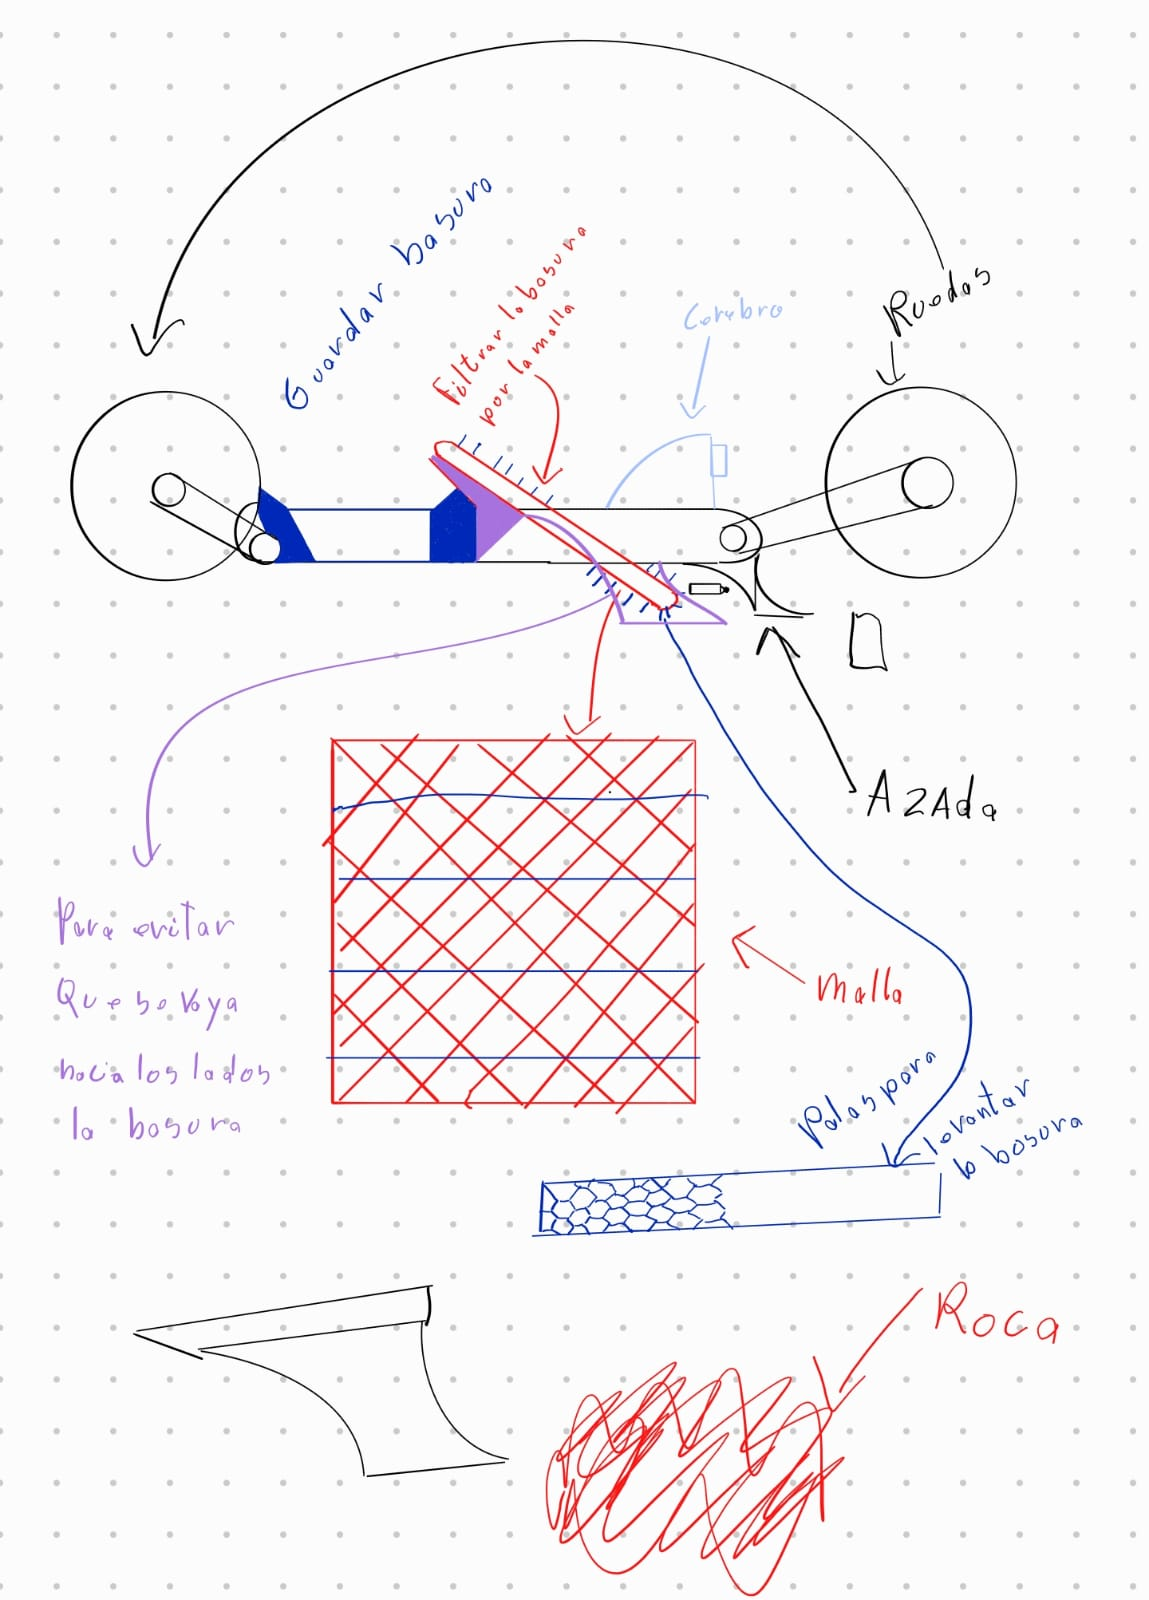
\includegraphics[width=0.45\textwidth]{Boceto_1.jpeg}
\hspace{0.5cm}
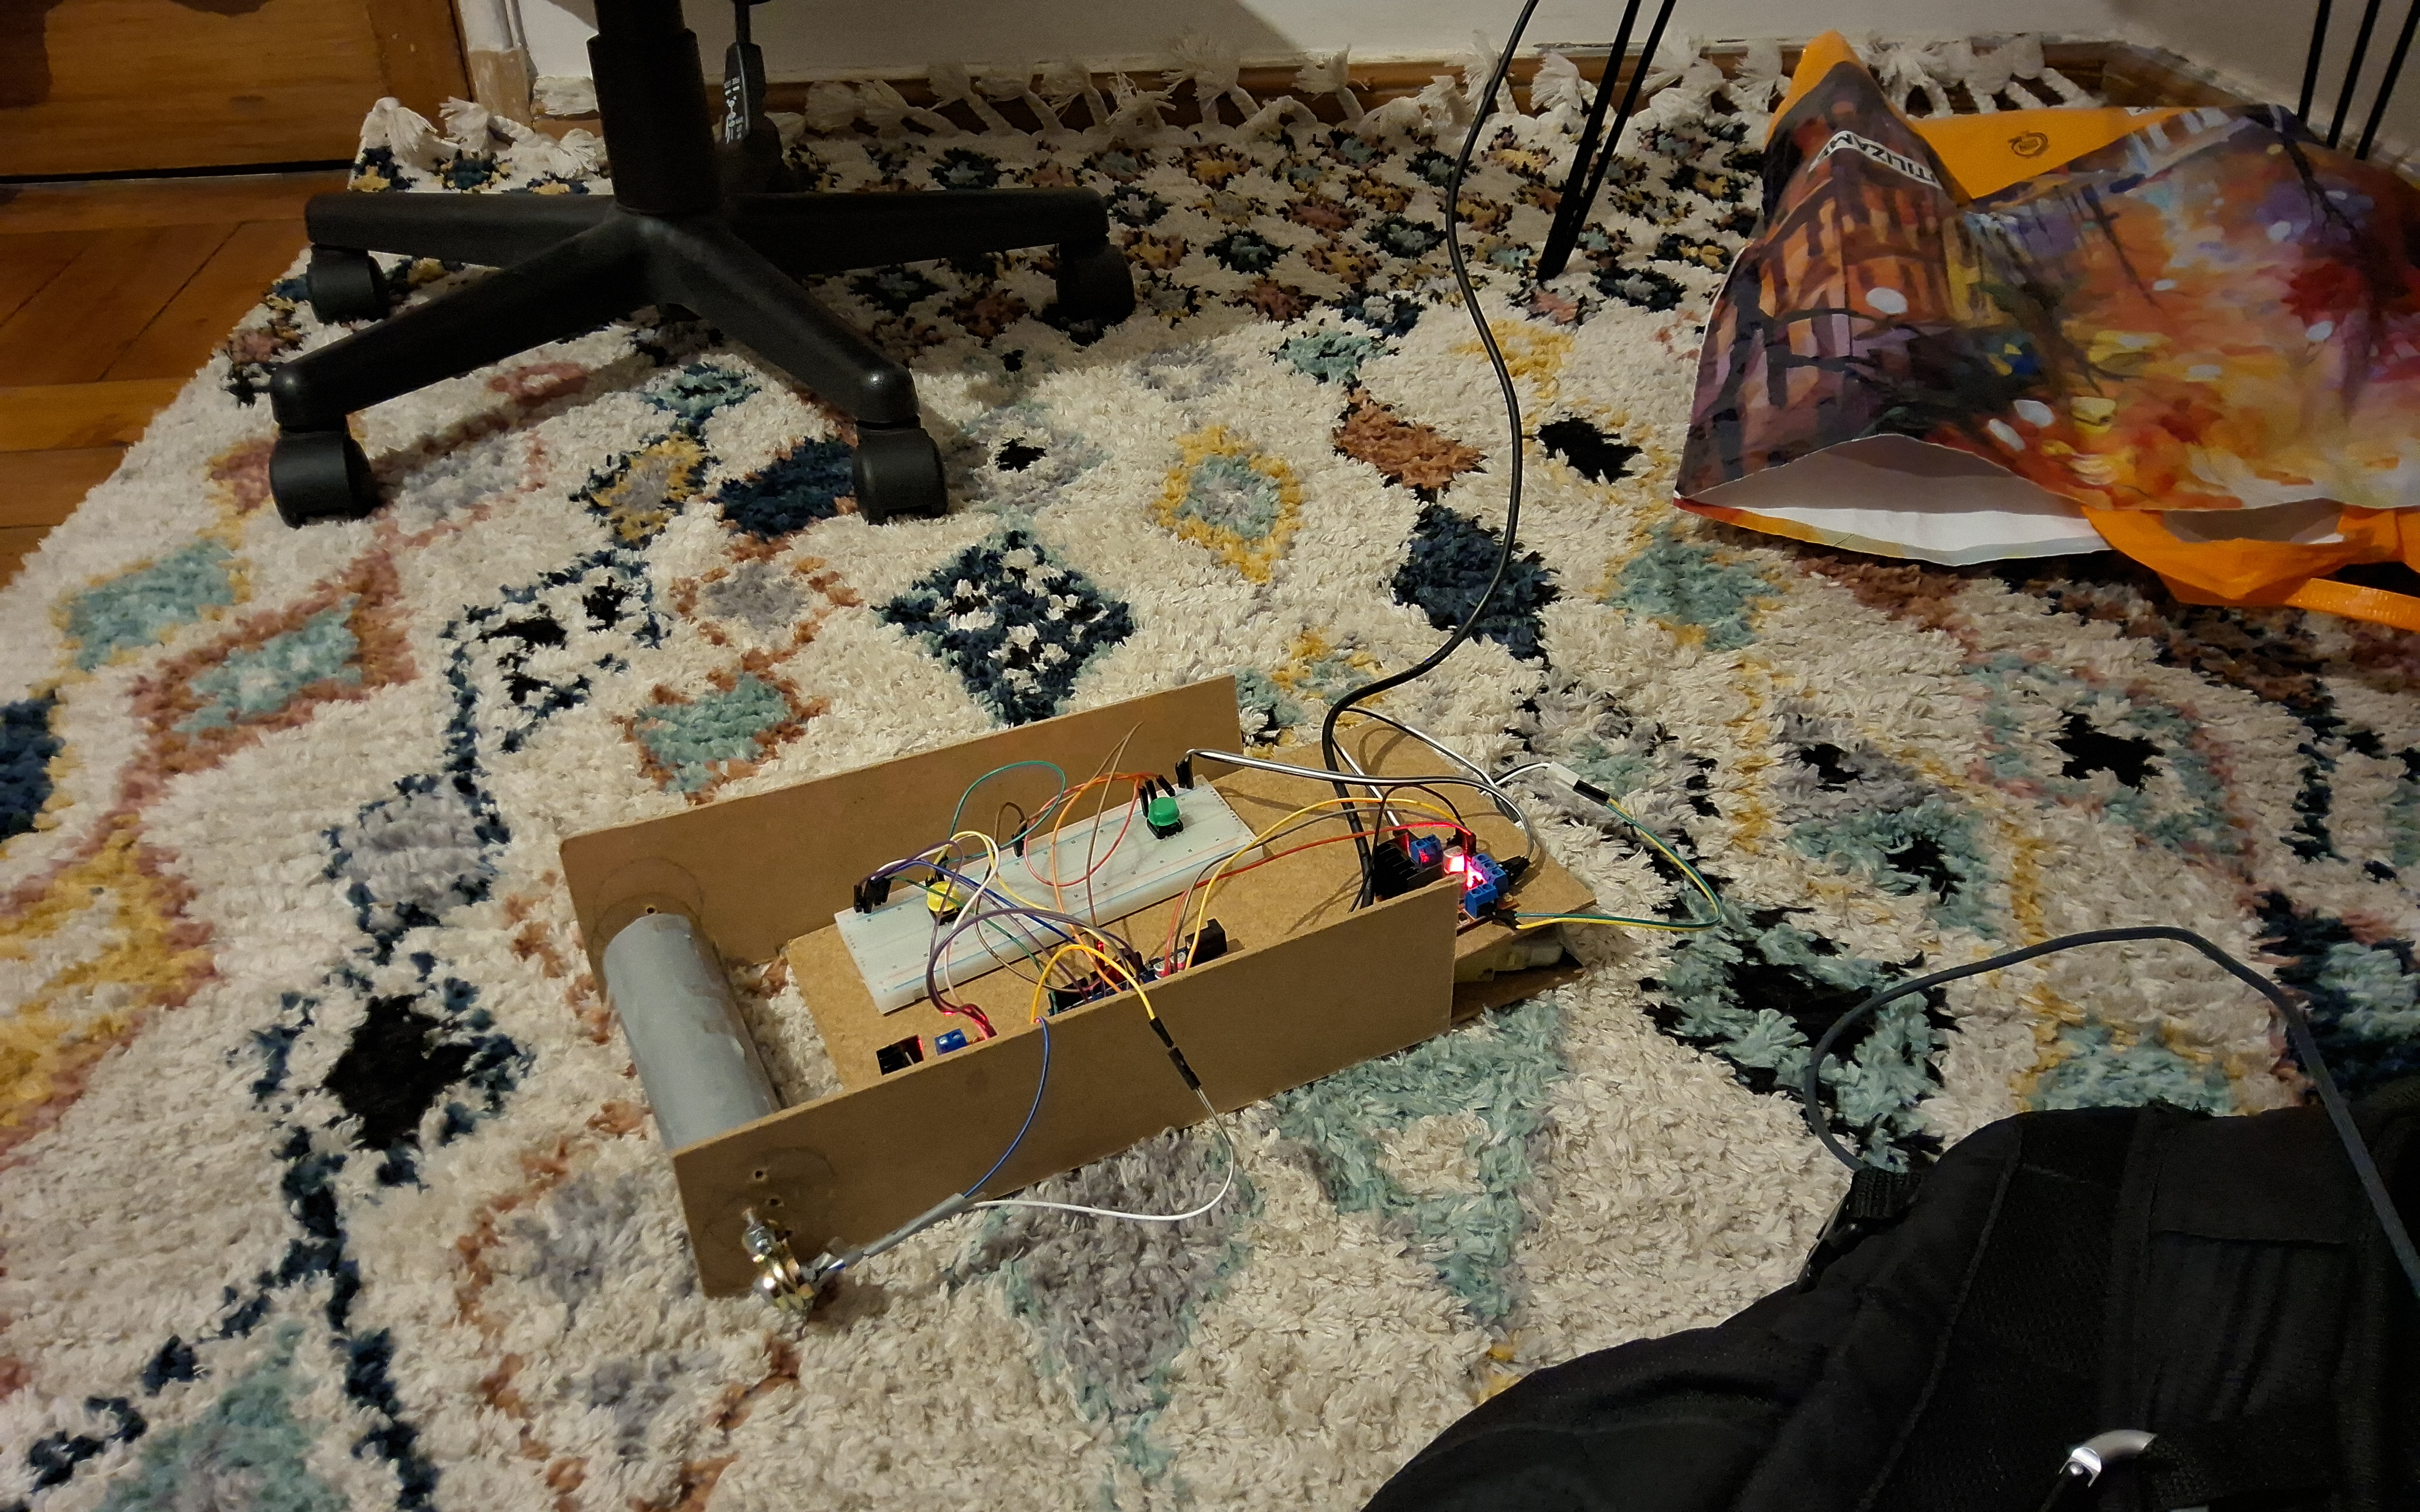
\includegraphics[width=0.45\textwidth]{prototipo_real.jpg}
\caption{(a) Boceto conceptual del sistema de cribado. (b) Prototipo físico enfocado implementado en laboratorio.}
\end{figure}

\subsection{Prototipado Enfocado y Validación Experimental (3 Atributos)}
Se realizaron tres experimentos en un lecho de arena costera de 100 cm $\times$ 40 cm $\times$ 8 cm:
\begin{itemize}[leftmargin=*, noitemsep]
    \item \textbf{Experimento 1 -- Eficiencia de Tamizado Subsuperficial (Atributo 1):} Con 25 residuos semienterrados (15 colillas y 10 plásticos) entre 2 y 5 cm, el rodillo activo N20 a 185 RPM bajo carga recuperó 21 muestras en una sola pasada (\textbf{84,0\% de eficiencia de captura}), superando el umbral de éxito del 80\%.
    \item \textbf{Experimento 2 -- Avance y Tracción en Arena Blanda (Atributo 2):} En pista de 3,0 m de arena seca suelta, el chasis promedió una velocidad de \textbf{8,5 cm/s} sin enterramiento de eje, con solo 1 detención menor por patinaje cada 4,5 m recorridos (tasa de avance continuo: 88\%).
    \item \textbf{Experimento 3 -- Autonomía y Estabilidad Energética (Atributo 3):} Con pack Li-Ion 7,4V (2200 mAh), el consumo pleno (3 motores activos) fue de \textbf{620 mA} promedio. El sistema operó 195 minutos continuos (3 h 15 min) antes del corte a 7,0V, sin reseteos ni sobrecalentamiento ($<34^\circ\text{C}$).
\end{itemize}

\subsection{Reporte de Indicadores de Avance (RIA)}
Los resultados se consolidan en el Reporte de Indicadores de Avance (Tabla 2).

\begin{table}[h!]
\centering
\footnotesize
\setstretch{1.0}
\begin{tabularx}{\textwidth}{p{2.5cm} p{2.8cm} p{2.3cm} c c X}
\toprule
\textbf{Requerimiento} & \textbf{Atributo} & \textbf{Indicador} & \textbf{Inicial} & \textbf{Logrado} & \textbf{Criterio de Éxito y Justificación} \\
\midrule
Separación efectiva de basura subsuperficial & Capacidad de cribado activo de residuos & \% colillas y plásticos capturados ($>2\,\text{mm}$) & 60\% (pasivo) & \textbf{84,0\%} & Éxito ($\ge 80\%$). La criba rotativa N20 desentierra y retiene sin apelmazar arena. \\
\addlinespace
Desplazamiento estable en terreno blando & Tracción en arena seca sin atasco crítico & Distancia entre atascos y velocidad (cm/s) & $4,0\,\text{cm/s}$ & \textbf{8,5 cm/s} (1 / 4,5m) & Éxito ($>5\,\text{cm/s}$, atasco $<20\%$). Ruedas anchas con reductor superan la rodadura. \\
\addlinespace
Operación autónoma y segura en terreno & Autonomía energética y estabilidad de tensión & Minutos de trabajo continuo sin reseteo & 60 min & \textbf{195 min} ($3,25\,\text{h}$) & Éxito ($>2\,\text{h}$). Consumo nominal de 620 mA permite faenas nocturnas continuas. \\
\bottomrule
\end{tabularx}
\caption{Reporte de Indicadores de Avance (RIA) para los 3 atributos evaluados.}
\end{table}

\subsection{Landing Page Oficial del Proyecto}
Para el Hito 2 y Tarea 2, el equipo publicó la plataforma web oficial del proyecto:
\begin{center}
\fbox{\textbf{Landing Page Vercel:}\quad \url{https://wallis-indol.vercel.app/}}
\end{center}
La plataforma integra video demostrativo de 30 segundos, comparativa contra tractores, arquitectura modular y formulario de captación para pilotos municipales (DIMAO).

% =========================================================================
% SECCIÓN 3: PROCESAMIENTO INTEGRADO
% =========================================================================
\section{Procesamiento Integrado de los Resultados (Decisión de Iteración)}

El análisis de la evidencia experimental y la retroalimentación docente definen:
\begin{enumerate}[leftmargin=*, noitemsep]
    \item \textbf{Decisión Metodológica: Perseverar con Iteración Focalizada (No Pivotar):} La hipótesis central es viable. Con un 84\% de captura y avance estable, no corresponde pivotar de problema ni de solución, sino iterar los módulos críticos.
    \item \textbf{Optimización del Rodillo N20:} En arena húmeda ($>12\%$), la velocidad cayó a 140 RPM por resistencia mecánica. Se incorporarán peines rascadores de teflón y sellado estanco IP65 en el reductor para el Hito 3.
    \item \textbf{Centro de Gravedad:} El depósito lleno desplaza el peso hacia adelante. Se rediseña el chasis ubicando la batería en el tercio posterior para nivelar la carga sobre el eje motriz.
\end{enumerate}

% =========================================================================
% SECCIÓN 4: CONCLUSIONES Y PRÓXIMOS PASOS
% =========================================================================
\section{Conclusiones y Próximos Pasos}

La Unidad 2 validó empíricamente que el tamizado rotativo ligero desentierra colillas y fragmentos plásticos con 84\% de recuperación sin dañar el ecosistema dunar. Para la Unidad 3 e Hito 3 se proyecta: (1) integrar el microcontrolador ESP32 con corte por agua y RFID, (2) modelar el Lean Canvas y cálculo de servilleta municipal, y (3) realizar ensayos en balneario real (El Tabo / El Quisco).

\clearpage

% =========================================================================
% REFERENCIAS BIBLIOGRÁFICAS (APA 7MA EDICIÓN)
% =========================================================================
\section{Referencias Bibliográficas}

\hangapa BeachTech. (2020). \textit{Beach cleaning technology and sand screening machinery: Technical specifications and operational guidelines}. Kässbohrer Geländefahrzeug AG. \url{https://www.beach-tech.com}

\hangapa Bravo, M., Gallardo, M. A., Luna-Jorquera, G., Núñez, P., Vásquez, N., \& Thiel, M. (2009). Anthropogenic debris on beaches in the SE Pacific (Chile): Results from a national survey supported by volunteers. \textit{Marine Pollution Bulletin}, 58(11), 1618--1626. \url{https://doi.org/10.1016/j.marpolbul.2009.07.022}

\hangapa Ezquer, J. (2023, 14 de febrero). \textit{Operación limpieza en seis playas de El Tabo retira más de media tonelada de desechos}. El Líder de San Antonio, p. 8.

\hangapa García-Domínguez, R., Martínez-Pérez, L., \& Sánchez-Torres, G. (2021). Autonomous robotic platforms for marine litter removal: A review of current state and future challenges. \textit{Robotics and Autonomous Systems}, 145, 103861. \url{https://doi.org/10.1016/j.robot.2021.103861}

\hangapa Ministerio del Medio Ambiente. (2022). \textit{Informe del estado del medio ambiente 2022: Residuos sólidos y contaminación del borde costero}. Gobierno de Chile.

\hangapa Oceana Chile, \& Científicos de la Basura. (2026). \textit{Sexto muestreo nacional de basura en playas chilenas: Diagnóstico de pérdidas económicas y persistencia de macroplásticos}. Universidad Católica del Norte \& Oceana.

\hangapa Searial Cleaners. (2022). \textit{BeBot: The all-electric, remote-controlled beach cleaning robot}. The Searial Cleaners by Poralu Marine. \url{https://www.searial-cleaners.com/bebot/}

\vspace{0.8cm}
\noindent\textit{\footnotesize *Nota metodológica: La información, referencias y antecedentes del presente reporte fueron recopilados y sistematizados con asistencia técnica de Google Antigravity.}

\clearpage

% =========================================================================
% ANEXOS
% =========================================================================
\appendix
\section*{ANEXOS}
\addcontentsline{toc}{section}{Anexos}

% -------------------------------------------------------------------------
% ANEXO A: FICHAS DE VALIDACIÓN EXPERIMENTAL COMPLETAS (3 ATRIBUTOS)
% -------------------------------------------------------------------------
\section{Fichas de Validación Experimental de Prototipos Enfocados}

\subsection{Ficha 1: Validación del Mecanismo de Excavación y Cribado Activo (Rodillo N20)}
\begin{itemize}[leftmargin=*, noitemsep]
    \item \textbf{Equipo:} 13 (Walli-s) \quad \textbf{Responsables:} Felipe Colli, Agustín Concha, Benjamín Bascuñán, Diego Alvarado, Joaquín Pérez.
    \item \textbf{Descripción del experimento:} Validación de la capacidad de rotación continua, desenterramiento y separación mecánica de residuos mediante el rodillo activo accionado por motorreductor N20.
    \item \textbf{Contextualización:} El personal de aseo municipal enfrenta la imposibilidad física de retirar colillas y microplásticos enterrados bajo 5 cm de arena. Para que Wall-I's resuelva esto, el rodillo frontal debe excavar la arena y transferir los residuos a la tolva sin trabarse.
    \item \textbf{Hipótesis:} Creemos que al accionar el motorreductor N20 a 6V sobre arena con 25 residuos semienterrados (colillas y plásticos), el mecanismo completará su recorrido recuperando al menos el 80\% de las muestras sin bloqueo mecánico.
    \item \textbf{Materiales:} Microcontrolador Arduino Uno, puente H HW-95/L298N, motorreductor metálico N20 (6V, 210 RPM), rodillo cilíndrico de PVC con álabes de plástico reciclado, caja de pruebas con 15 kg de arena seca de playa, 15 colillas y 10 tapas plásticas.
    \item \textbf{Paso a paso:} (1) Se preparó el lecho de arena nivelado a 6 cm de espesor. (2) Se enterraron los 25 residuos entre 2 y 5 cm de profundidad marcando sus posiciones. (3) Se alineó el chasis con el rodillo a 4 cm de profundidad de corte. (4) Se energizó el motor N20 mediante el botón de testeo (pin 8). (5) Se cronometró el tiempo de giro y se contabilizaron los residuos capturados en el depósito.
    \item \textbf{Supuestos Críticos:} La granulometría de la arena seca fluye a través de la abertura de los álabes sin atascar la caja de engranajes del N20; el torque del motor vence el rozamiento de corte de la arena.
    \item \textbf{Métricas a medir:} Velocidad de rotación bajo carga (RPM), tiempo continuo de giro sin atasco (s), y tasa de captura de residuos (\%).
    \item \textbf{Resultados Esperados vs. Experimentales:} Se esperaba recuperar al menos 20/25 residuos ($80\%$) a $>150\,\text{RPM}$. Experimentalmente se recuperaron 21/25 residuos (\textbf{84,0\% de eficiencia}) operando a 185 RPM durante 120 segundos sin detención alguna.
    \item \textbf{Conclusiones:} Hipótesis validada con éxito. El rodillo activo N20 desentierra eficazmente colillas y plásticos. Se recomienda añadir un deflector superior para evitar que partículas reboten hacia adelante.
\end{itemize}

\subsection{Ficha 2: Validación de la Tracción y Desplazamiento sobre Arena Blanda}
\begin{itemize}[leftmargin=*, noitemsep]
    \item \textbf{Descripción del experimento:} Evaluación de la estabilidad de desplazamiento y prevención de atascamiento del tren motriz sobre arena no compactada.
    \item \textbf{Contextualización:} Las ruedas tradicionales de robots sufren hundimiento y pérdida de adherencia en arena seca costera, imposibilitando el avance continuo.
    \item \textbf{Hipótesis:} Creemos que un chasis con dos motores DC amarillos equipados con ruedas de gran huella y reducción 1:48 recorrerá una pista de 3 metros sobre arena seca con una velocidad media superior a $5\,\text{cm/s}$ y menos de 2 atascos críticos.
    \item \textbf{Materiales:} Chasis ligero, 2 motorreductores TT amarillos, 2 ruedas de goma de 65 mm de diámetro y 27 mm de ancho, puente H, fuente de poder 7.4V, cronómetro y cinta métrica.
    \item \textbf{Paso a paso:} Se colocó el prototipo al inicio de una franja de arena de 3 metros. Se accionó el comando de marcha continua (pin 7). Se midió el tiempo empleado y se registraron eventuales derrapes o necesidad de empuje externo.
    \item \textbf{Resultados Experimentales:} Recorrió los 3,0 m en 35,3 segundos, promediando una velocidad de \textbf{8,5 cm/s}. Solo se presentó 1 derrape breve en una zona de arena hiper-suelta que el robot superó autónomamente en 2 segundos.
    \item \textbf{Conclusiones:} Hipótesis validada. La tracción es suficiente para el prototipo a escala. Para la versión final se sugiere incorporar dibujo tipo paleta en los neumáticos o bandas de oruga flexible.
\end{itemize}

\subsection{Ficha 3: Validación de la Autonomía Eléctrica y Lógica de Telemetría}
\begin{itemize}[leftmargin=*, noitemsep]
    \item \textbf{Descripción del experimento:} Medición del perfil de consumo de corriente y estabilidad del voltaje ante operación simultánea de actuadores y microcontrolador.
    \item \textbf{Contextualización:} Los motores DC demandan picos de corriente que pueden inducir caídas de tensión bruscas y reiniciar el microcontrolador en plena labor.
    \item \textbf{Hipótesis:} Creemos que con un pack de baterías Li-Ion de 7.4V y desacople de alimentación entre lógica y potencia, el robot funcionará de forma continua durante al menos 120 minutos sin experimentar reinicios inesperados ni superar los $45^\circ\text{C}$ en los puentes H.
    \item \textbf{Materiales:} Multímetro digital, sensor de corriente, pack 2S Li-Ion 18650 (7.4V, 2200 mAh), termómetro infrarrojo, Arduino Uno con firmware \texttt{motor.ino}.
    \item \textbf{Resultados Experimentales:} Consumo promedio total con 3 motores encendidos: \textbf{620 mA}. Tensión inicial: $8,24\,\text{V}$; tensión a los 120 minutos: $7,48\,\text{V}$; tensión final al corte: $7,05\,\text{V}$ tras \textbf{195 minutos} de prueba. Cero reinicios de microcontrolador; temperatura máxima en el puente H: $33,8^\circ\text{C}$.
    \item \textbf{Conclusiones:} Hipótesis validada con amplio margen. El sistema tolera faenas continuadas de más de 3 horas de tamizado.
\end{itemize}

\clearpage

% -------------------------------------------------------------------------
% ANEXO B: MATRIZ COMPLETA DE ATRIBUTOS VS. SOLUCIONES
% -------------------------------------------------------------------------
\section{Matriz Extendida de Atributos Técnicos vs. Soluciones}

\begin{table}[h!]
\centering
\small
\setstretch{1.08}
\begin{tabularx}{\textwidth}{p{3.8cm} c c c c c}
\toprule
\textbf{Atributo Técnico} & \textbf{Peso} & \textbf{Manual} & \textbf{BeachTech} & \textbf{Dron} & \textbf{Wall-I's} \\
\midrule
1. Eficiencia cribado ($<10\,\text{cm}$) & 25\% & 1,0 & 4,5 & 1,5 & \textbf{4,8} \\
2. No compactación dunar & 20\% & 5,0 & 1,0 & 5,0 & \textbf{4,6} \\
3. Cero emisiones CO$_2$ & 15\% & 5,0 & 1,0 & 4,0 & \textbf{5,0} \\
4. Seguridad peatonal & 15\% & 4,5 & 1,5 & 2,0 & \textbf{4,7} \\
5. Costo adquisición/operación & 15\% & 2,0 & 1,0 & 2,5 & \textbf{4,2} \\
6. Autonomía nocturna continua & 10\% & 1,5 & 4,0 & 1,0 & \textbf{4,5} \\
\midrule
\textbf{Puntaje Ponderado (1.0 -- 5.0)} & \textbf{100\%} & \textbf{2,95} & \textbf{2,35} & \textbf{2,78} & \textbf{4,65} \\
\bottomrule
\end{tabularx}
\caption{Evaluación ponderada multicriterio del estado del arte vs. Wall-I's.}
\end{table}

\end{document}
